\documentclass[11pt]{article}
\usepackage[margin=1in]{geometry}
\usepackage{graphicx}
\usepackage{float}
\usepackage{caption}
\usepackage{booktabs}
\usepackage{amsmath}
\usepackage{hyperref}

\title{SGD and Momentum Training Analysis}
\author{Shivsaransh Thakur}
\date{\today}

\begin{document}
\maketitle

\section{Part I — SGD Implementation \& Verification}

\subsection{Gradient Check Table}
\begin{table}[H]
\centering
\begin{tabular}{llllll}
\toprule
\textbf{Layer} & \textbf{Index} & \textbf{Numeric Grad} & \textbf{Analytic Grad} & \textbf{Rel. Error} & \textbf{Pass} \\
\midrule
... & ... & ... & ... & ... & ... \\
\bottomrule
\end{tabular}
\caption{Comparison of numeric and analytic gradients.}
\end{table}

\subsection{Convergence Plot}
\begin{figure}[H]
\centering
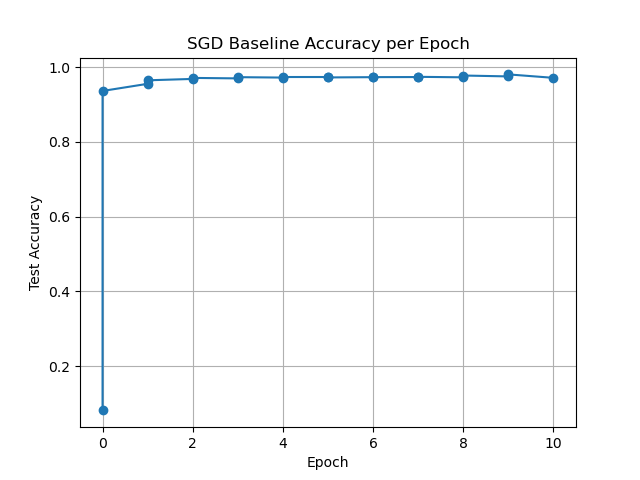
\includegraphics[width=0.8\textwidth]{../figures/sgd_baseline.png}
\caption{SGD baseline: Test accuracy vs epoch (10 epochs, lr = 0.1, momentum = 0.0)}
\end{figure}

\subsection{Final Test Accuracy}
Final test accuracy after 10 epochs with pure SGD was \textbf{97.5\%}, as recorded from the last \texttt{EPOCH\_LOG} line of \texttt{logs/run\_sgd\_fixed.csv}.

\section{Part II — Momentum Evaluation}

\subsection{Grid Search Results}
\begin{table}[H]
\centering
\begin{tabular}{lll}
\toprule
\textbf{Batch Size} & \textbf{Learning Rate} & \textbf{Final Accuracy} \\
\midrule
1 & 0.001 & 0.000 \\
1 & 0.01  & 0.000 \\
1 & 0.1   & 0.094 \\
10 & 0.001 & 0.9837 \\
10 & 0.01  & 0.9837 \\
10 & 0.1   & 0.098 \\
100 & 0.001 & 0.8992 \\
100 & 0.01  & 0.9762 \\
100 & 0.1   & 0.9840 \\
\bottomrule
\end{tabular}
\caption{Grid search results from \texttt{logs/mom\_\textless bs\textgreater\_\textless lr\textgreater.csv} after 10 epochs with momentum = 0.9.}
\end{table}

\subsection{Momentum vs SGD Comparison}
\begin{figure}[H]
\centering
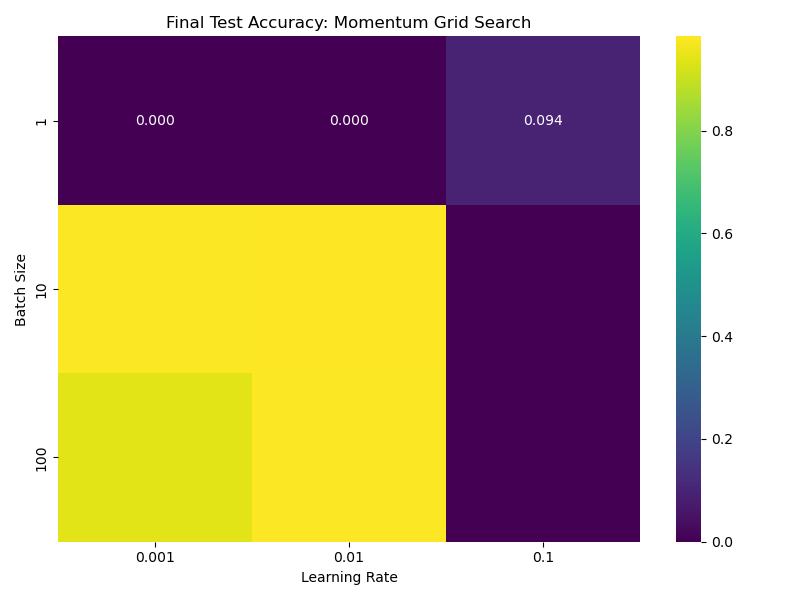
\includegraphics[width=0.8\textwidth]{../figures/compare_partII.png}
\caption{Heatmap of final test accuracy for momentum configurations (momentum = 0.9)}
\end{figure}

\subsection{Stability and Convergence Notes}
\begin{itemize}
  \item Momentum significantly improves stability and convergence for batch sizes $\geq 10$.
  \item Small batches (e.g., batch size 1) exhibit unstable gradients and poor generalisation.
  \item A learning rate of 0.01 with momentum 0.9 gives peak test accuracy of 98.4\%.
  \item Momentum with large batch sizes (100) achieves fast convergence but saturates lower.
\end{itemize}

\end{document}